The proposed competition is a regression problem about age estimating, in fact based on vocal recordings and some informatoon regarding the person, such as his ethnicity and his gender, we aim to correctly determine the age of the person who is talking.
The dataset is divided in two parts:
\begin{itemize}
    \item a \emph{development} set, containing $2933$ elements, each of them labeled  
    \item an \emph{evaluation} set, containing $691$ elements
\end{itemize}
The development set will be used to build a regressor to label the elements of the evaluation set.

We can make some considerations based on the development set. First, the dataset is complete, indeed non of the rows contains missing values. 
Second, some features requires some preprocessing: \emph{ethnicity} and \emph{gender} are a categorial features and, thus, they need to be encoded in order to be used in the regression; \emph{tempo} is not automatically saved as a float type because the values are enclosed by parenthesis.
Third, the dataset also contains the path to the vocal recordings from which we have decided to extract more features from the spectogram.

We can study the correlation of the feature given by the dataset by analizing the correlation plot shown in figure $\eqref{correlation_plot}$.
\begin{figure}
    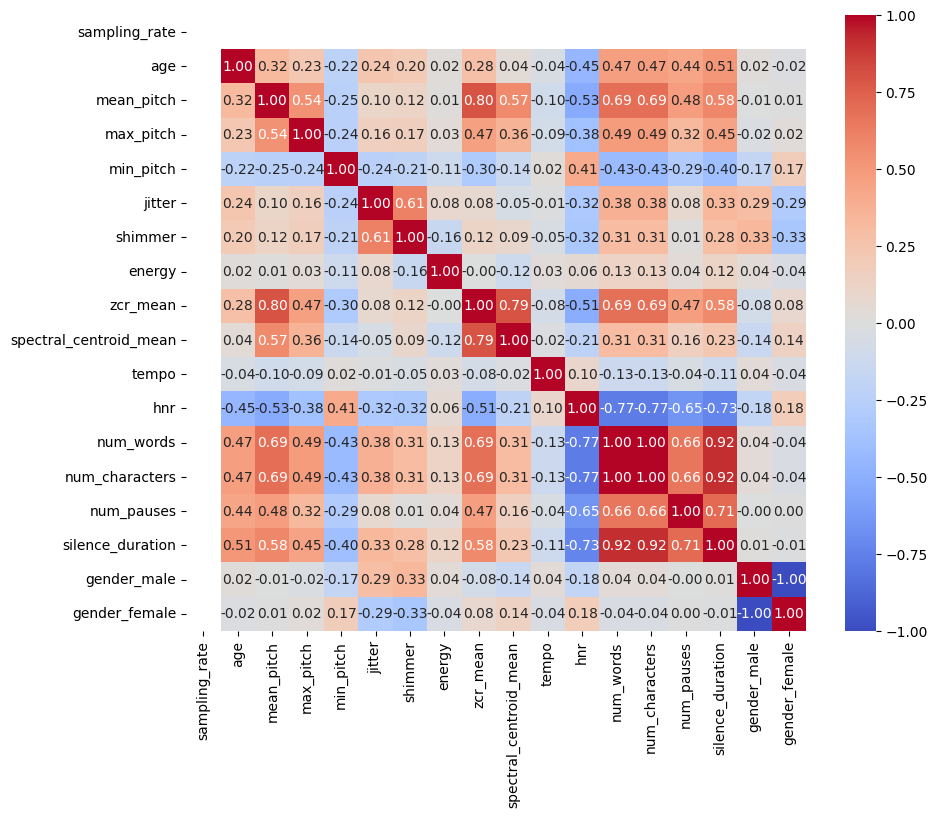
\includegraphics[width = 0.47\textwidth]{img/correlation_plot.png}
    \caption{Correlation among features.}
    \label{correlation_plot}
\end{figure}

To better understand the distribution of the features we can plot some histograms.
From the histograms shown in figure $\eqref{hist_distributivi}$ we can notice that most of the features seems to be distributed as Gaussian distribution with not many outliers. 
Some exceptions are \textit{max\_pitch}, \textit{min\_pitch} and \textit{num\_characters}: the first two features mentioned have a very wide range of values but almost all their distribution mass is concentrated in a single point, thus there are many outliers; on the contrary, \textit{num\_characters} concentrates his mass distribution in two far values.

\begin{figure}
    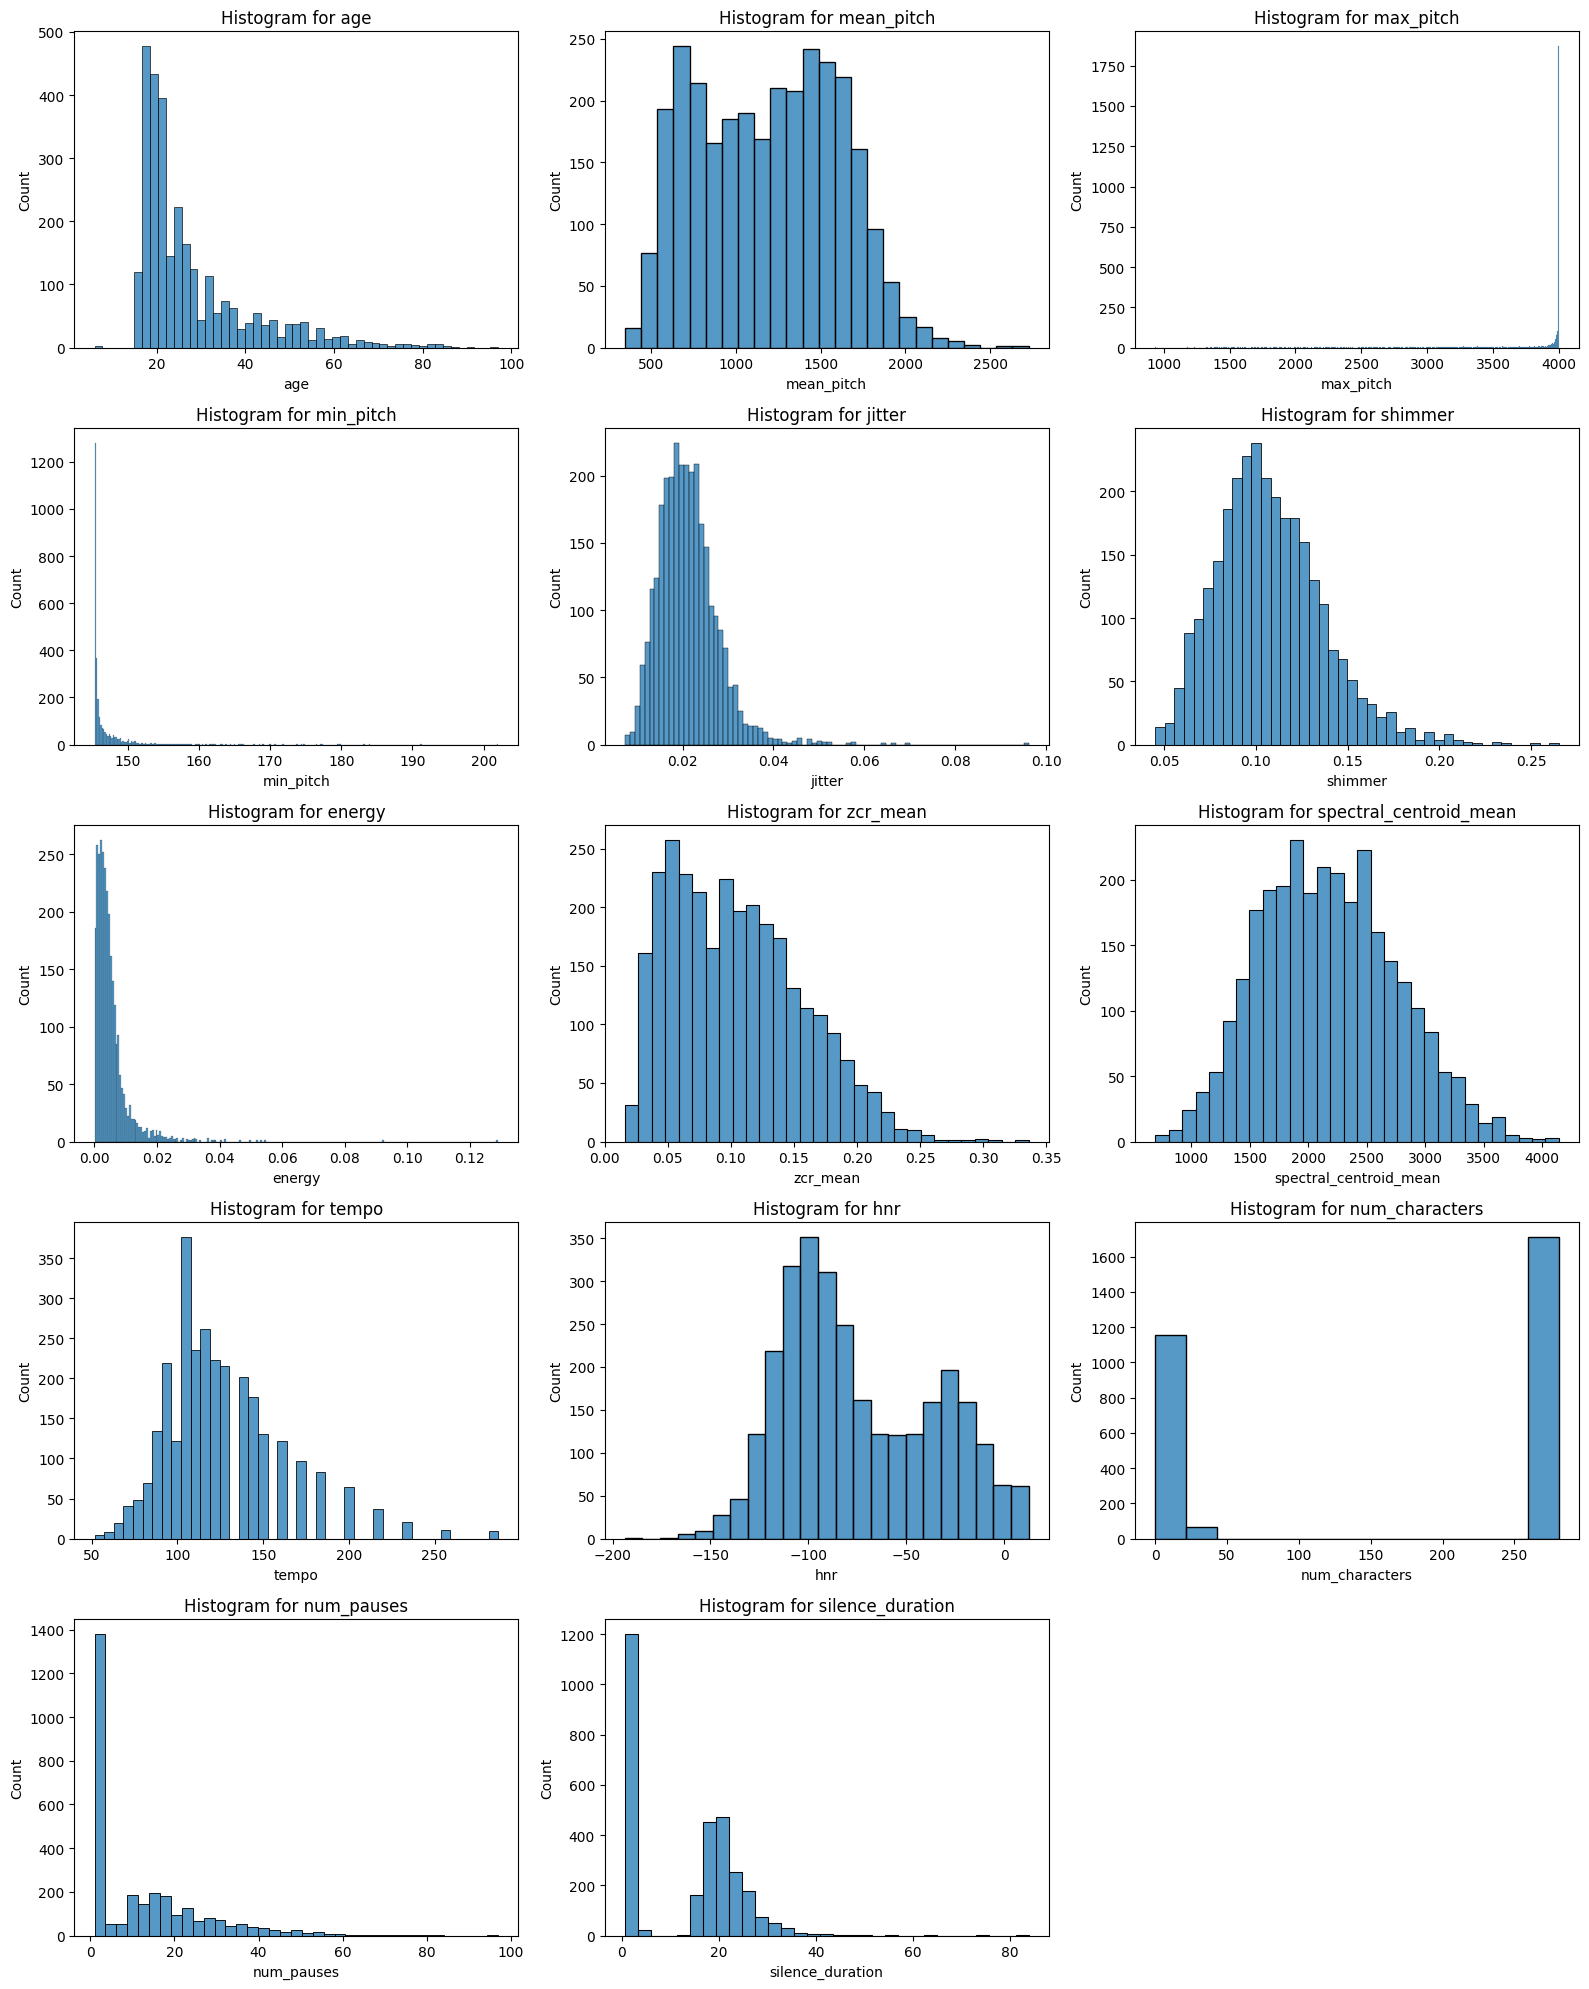
\includegraphics[width = 0.47\textwidth]{img/distribuzioni_features.png}
    \caption{Histograms of some features.}
    \label{hist_distributivi}
\end{figure}